%开普勒第二定律的证明

\pentry{开普勒第二定律\upref{Keple}, 角动量守恒(单个质点)\upref{AMLaw1}}
\begin{figure}[ht]
\centering
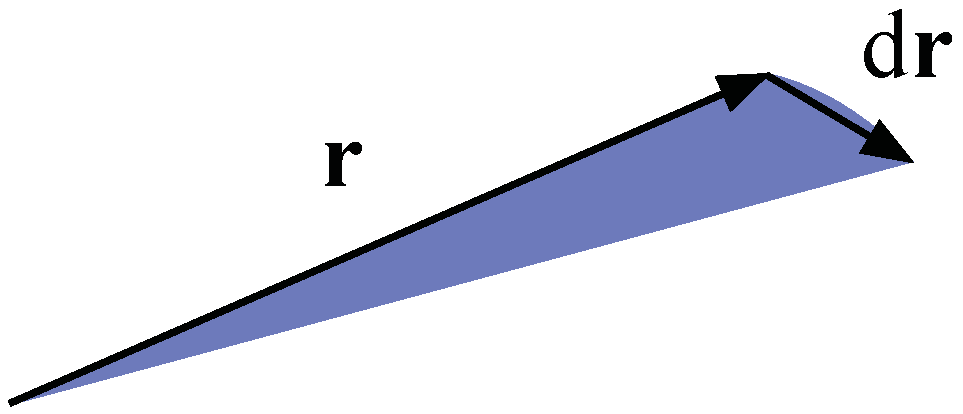
\includegraphics[width=4.5cm]{./figures/Keple21.pdf}
\caption{微小时间 $\D t$ 扫过的面积} \label{Keple21}
\end{figure}

令行星的位矢为 $\vec r$,  在很小一段时间 $\D t$ 内移动了 $\D \vec r$,  于是扫过的面积就是以 $\vec r$ 和 $\D \vec r$ 为两条边的三角形的面积 $\D S = {1}/{2}\left| {\vec r} \right| \cdot \left| {\D \vec r} \right|\sin \theta $,  其中 $\theta $ 为两条矢量的夹角.若把面积看成矢量, 方向垂直于三角形所在的平面, 则根据叉乘的定义有 $\D \vec S = \vec r \cross \D \vec r/2$. 两边除以 $\D t$,  得扫过面积的速率为
\begin{equation}
  \frac{{\D\vec S}}{{\D t}} = \frac{1}{2}\vec r \cross \frac{{\D\vec r}}{{\D t}} = \frac 12 \vec r\cross \vec v
\end{equation}
由“角动量守恒\upref{AMLaw1}”, 行星角动量不变.
$\vec r \cross \left( {m\vec v} \right) = \vec L$ (常矢量, 垂直运动平面) 所以 ${{\D\vec S}}/{{\D t}} = {{\vec L}}/{{2m}}$ 也是常矢量.写成标量形式, 即
\begin{equation}
  \frac{{\D S}}{{\D t}} = \frac{L}{{2m}}
\end{equation}
所以从任意时刻 ${t_0}$ 开始, 在一段时间 $\Delta t$ 内行星扫过的面积为 
\begin{equation}
  \begin{aligned}
  \Delta S = \frac{L}{{2m}}\Delta t
  \end{aligned}
\end{equation}
只和时间间隔有关, 而与起始位置无关.

